\chapter{Numerical Implementation}
\label{app:numerical-implementation}

The numerical implementation of the self-consistent equations was performed mainly
in \verb|Python 3.9| and partially in \verb|Mathematica|. Some of the numerical methods are inspired by the work of J. Winkel in our group, see~\cite{Winkel2021} for more details. The main steps and ideas of the present numerical framework are:

\begin{enumerate}
\item First iteration of the boson propagator: \\
Start with the analytic expression for $\text{Im}\,\Pi^R_{\phi}$ and calculate $\text{Re}\,\Pi^R_{\phi}$ on a finite grid. To simplify the calculation, treat the divergent vacuum part analytically, see below. \\
Choose grid size large enough such that the numerical corrections are quite small. This can be quantified in dependence of the temperature.
\item First iteration of the fermion propagator: \\
Take the bare fermion spectral function (delta peak) and the semi-analytic boson spectral function from the first iteration and calculate $\text{Im}\,\Sigma^R_{\psi}$ with~\eqref{eq:imaginary-part-self-energies} on a finite grid. From this, obtain $\text{Re}\,\Sigma^R_{\psi}$ as described below.
\item Further iterations of the fermion propagator: \\
Take the numerical spectral functions for the fermion and boson and calculate the self-energy as in step 2.
\item Further iterations of the boson propagator: \\
Take numerical spectral functions for the fermions and calculate $\text{Im}\,\Pi^R_{\phi}$ on a finite grid. Outside the grid, glue smoothly to the analytical non-selfconsistent result. Compute the difference $\delta\text{Re}\,\Pi^R_{\phi}$ to the non-selfconsistent result.
\end{enumerate}

For the numerical calculation of 2-dimensional functions an adaptive python package, called \verb|Adaptive|~\cite{Nijholt2019}, is used. The sampling points are chosen automatically based on the functional form. Less samples are taken in smoother regions and more samples are taken in faster changing regions. Additionally, the calculation of these sampling points can be parallelized over multiple cores. An example of how sampling points are taken by \verb|Adaptive| is shown in Fig.~\ref{fig:adaptive}. The resulting sampling points are then linearly interpolated. It is useful to simplify the interpolation by deforming the functions onto the quadratic dispersion relation, see Fig.~\ref{fig:shift_dispersion}. For the bosonic self-energy, this step can significantly improve the resolution of sharp edges in the function. For the fermionic self-energy, it can additionally help to ensure a large enough distance of the grid boundary to the main peak, such that asymptotic behavior is visible. 

The numerical integration of the self-energy loop integrals is performed mainly with an adaptive Monte Carlo method from \verb|Vegas+|~\cite{Lepage2021}. This allows for maximal flexibility when dealing with highly peaked integrands in a multidimensional space and can be generalized easily. However, this comes with the downside of a long runtime. For this specific use case, a different adaptive integration routine using sparse grids might be more efficient. The 1-dimensional principal value integral for the real part of the self-energy is computed using the adaptive quadrature integration from \verb|SciPy|~\cite{Virtanen2019}.

\begin{figure}[h]
	\centering
	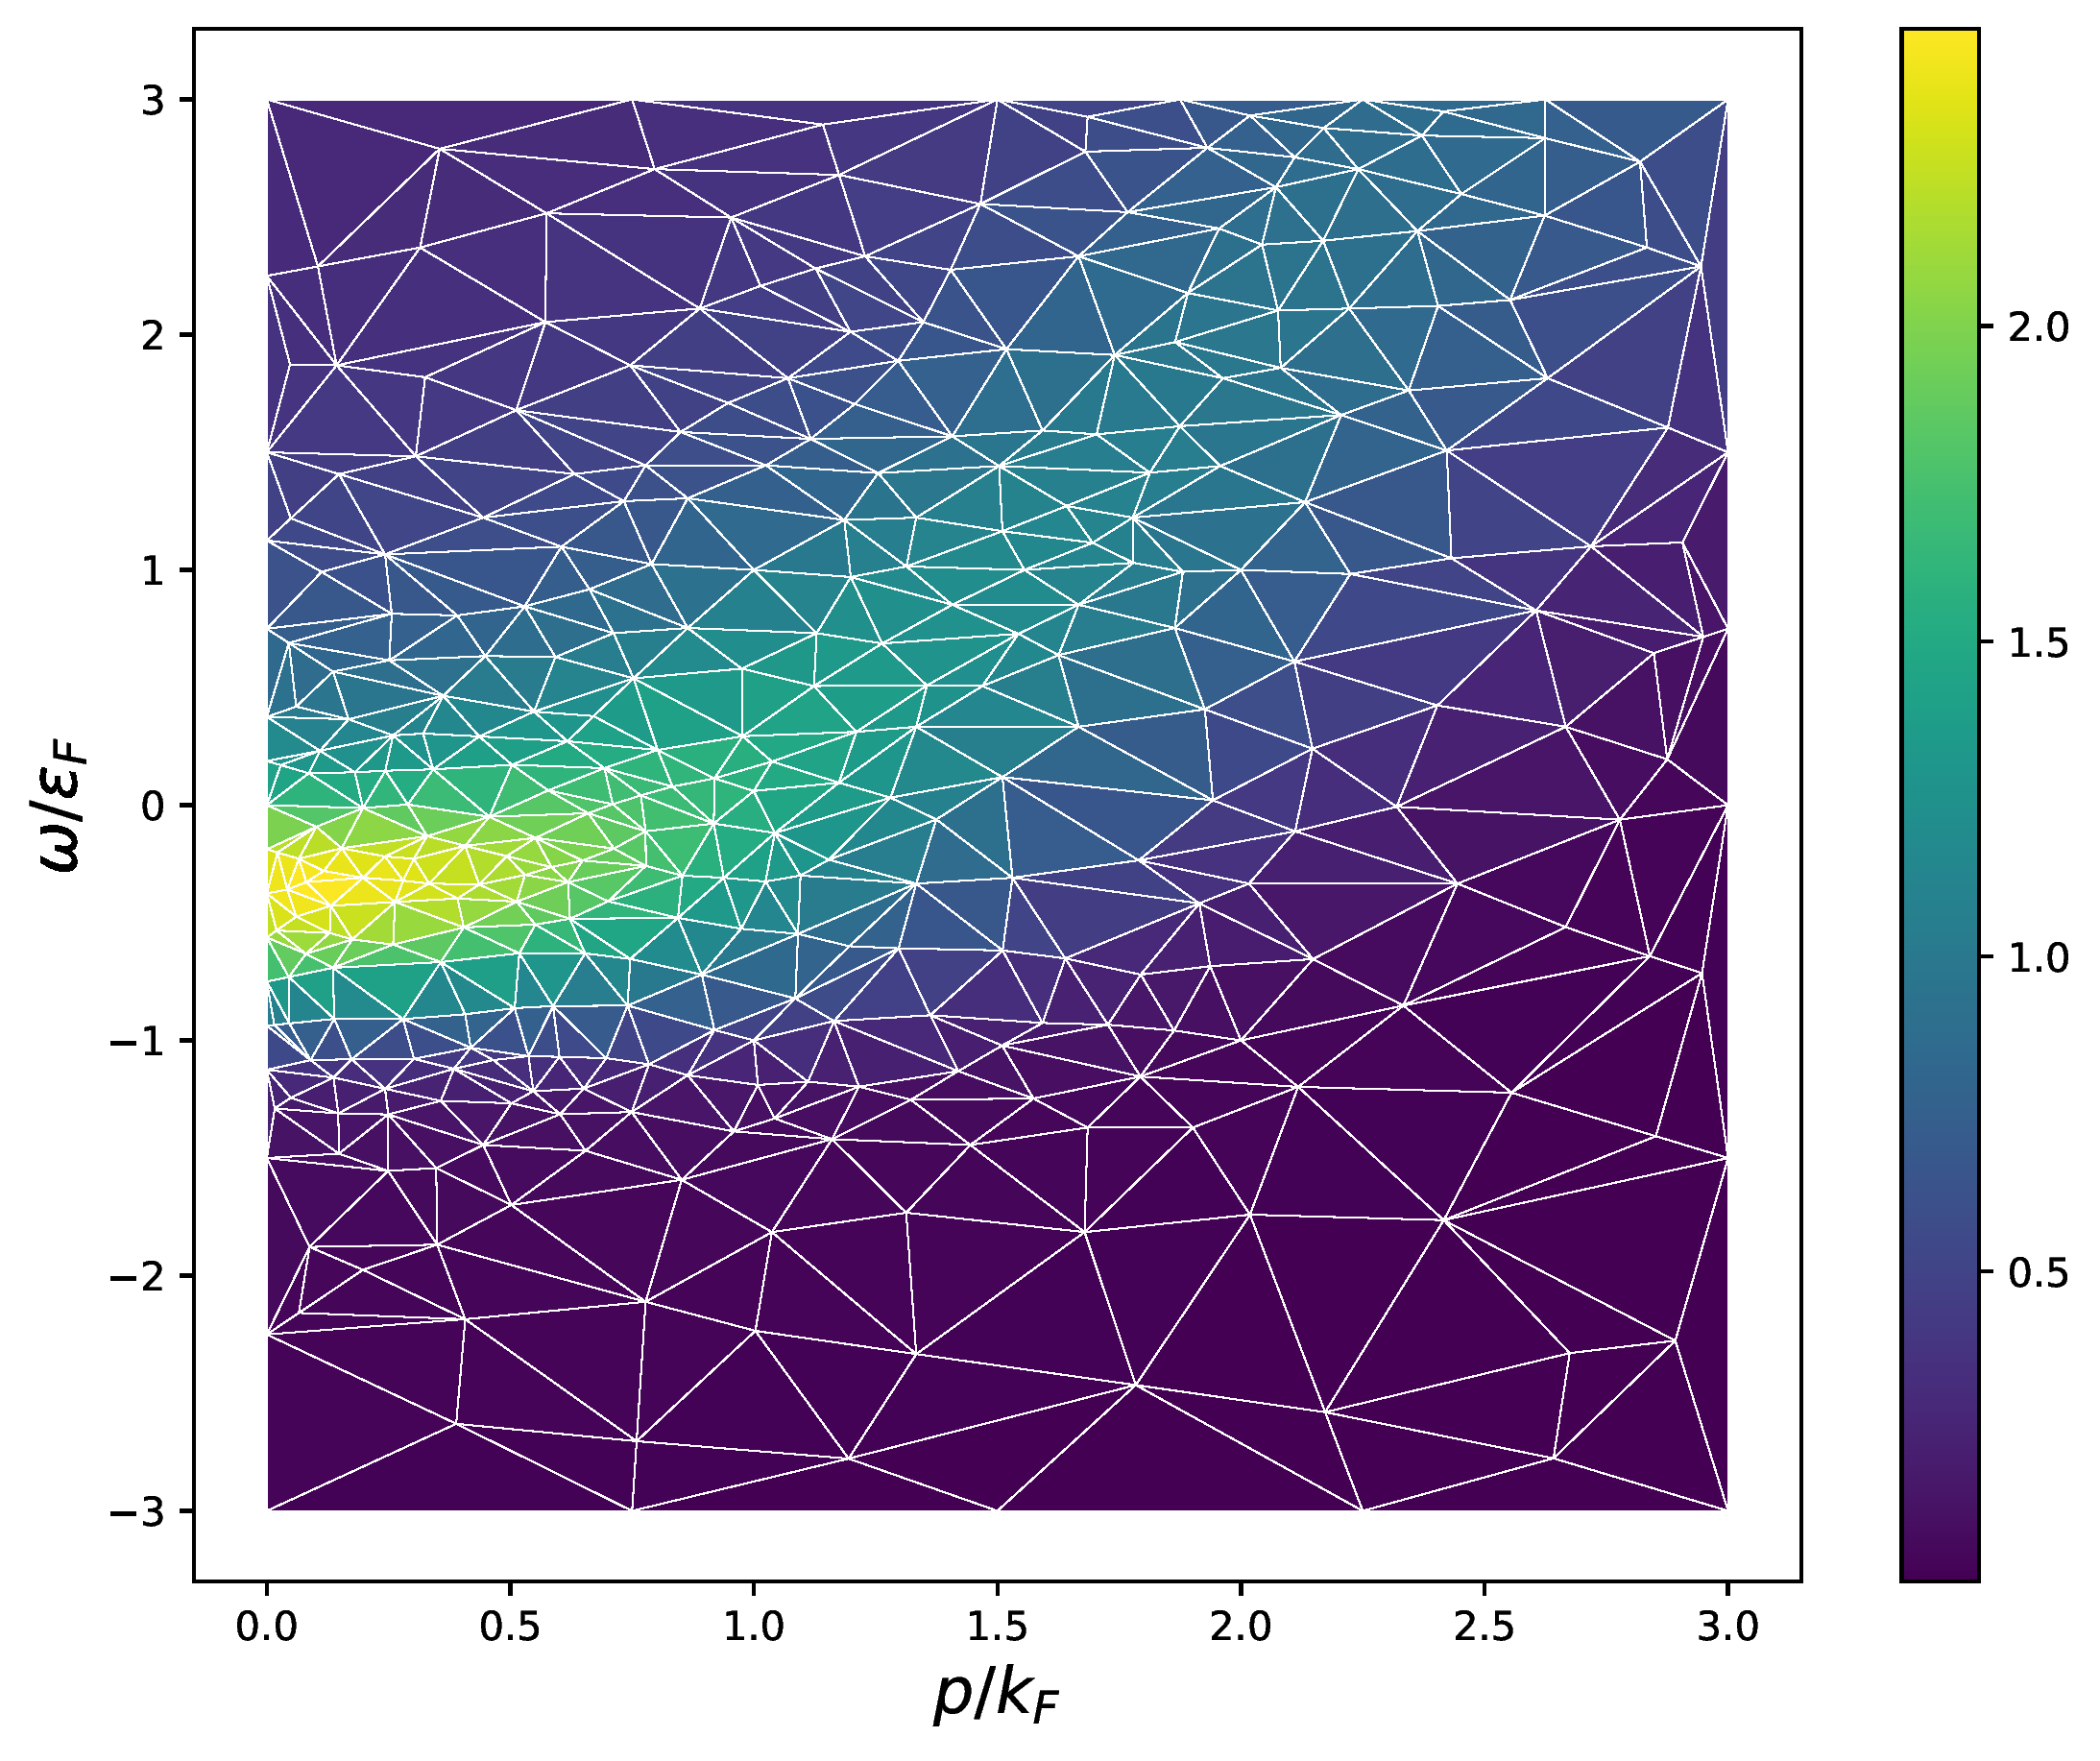
\includegraphics[width=0.58\textwidth]{figs/adaptive.png}
	\caption[Evaluation of a function with Adaptive]{Example of a 2-dimensional function evaluated by Adaptive.}
	\label{fig:adaptive}
\end{figure}

\begin{figure}[h]
	\centering
	\subfigure[]{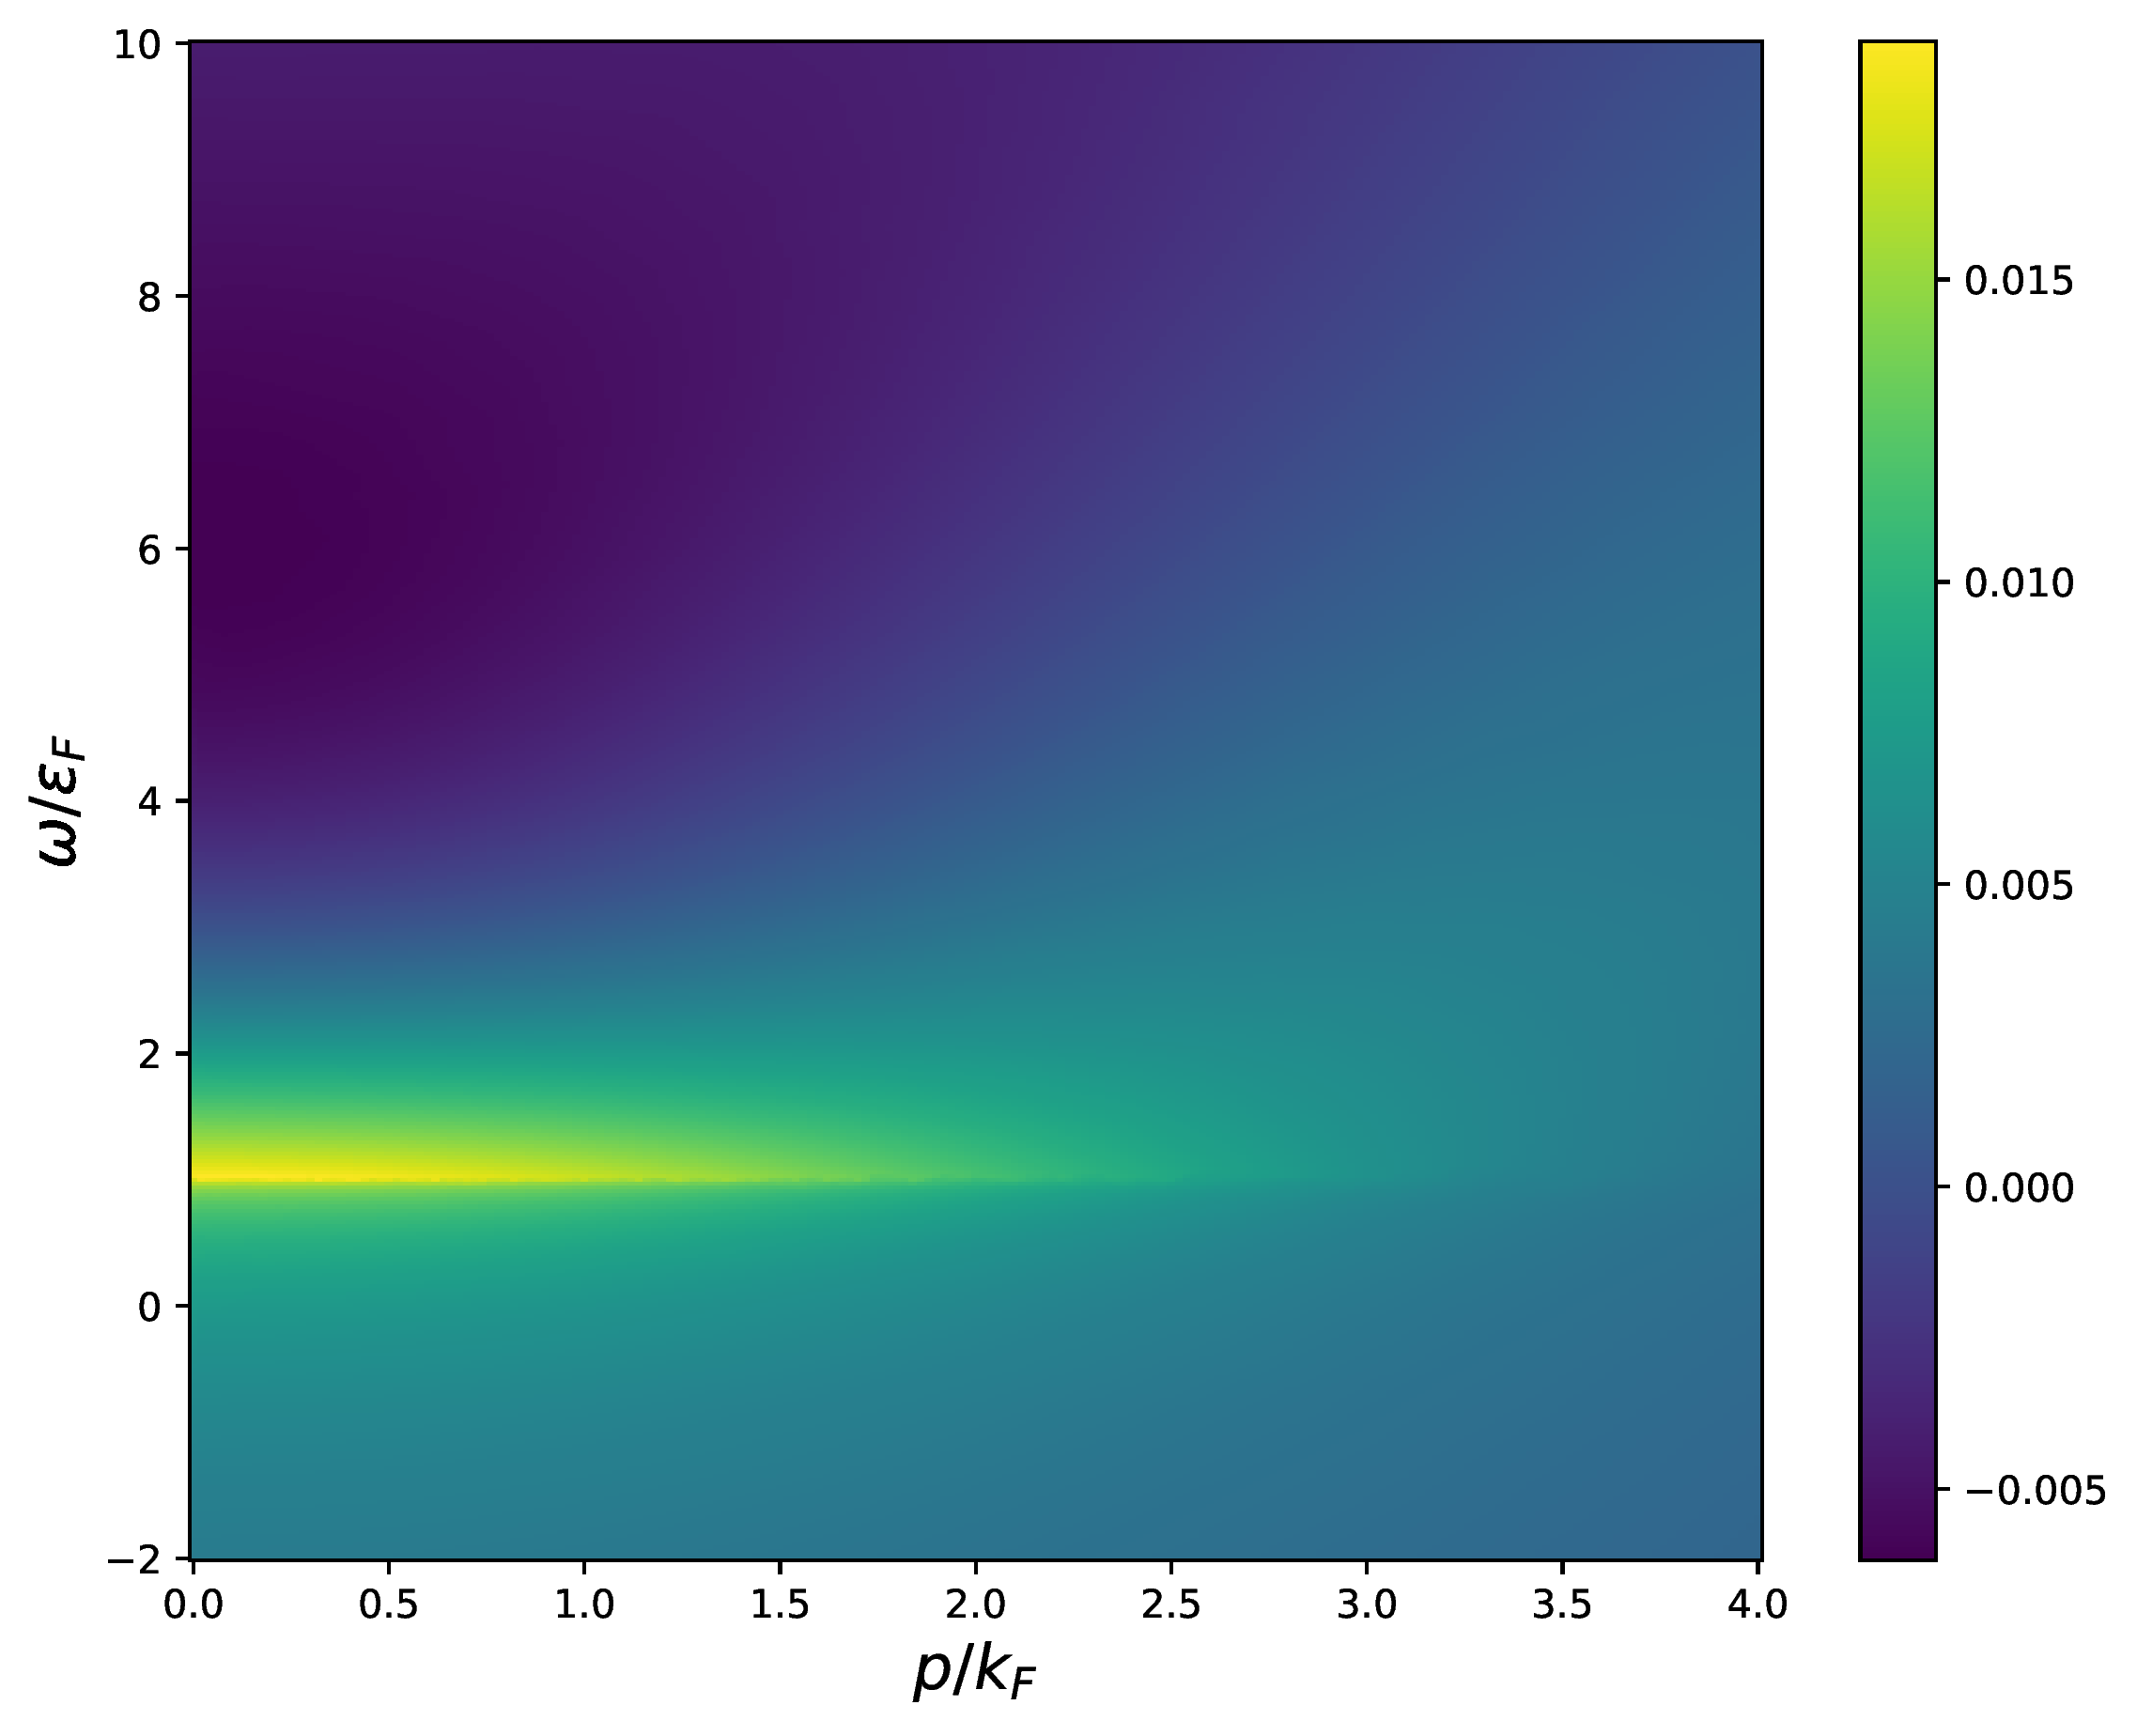
\includegraphics[width=0.46\textwidth]{figs/dispersion-shift1.png}} 
	\subfigure[]{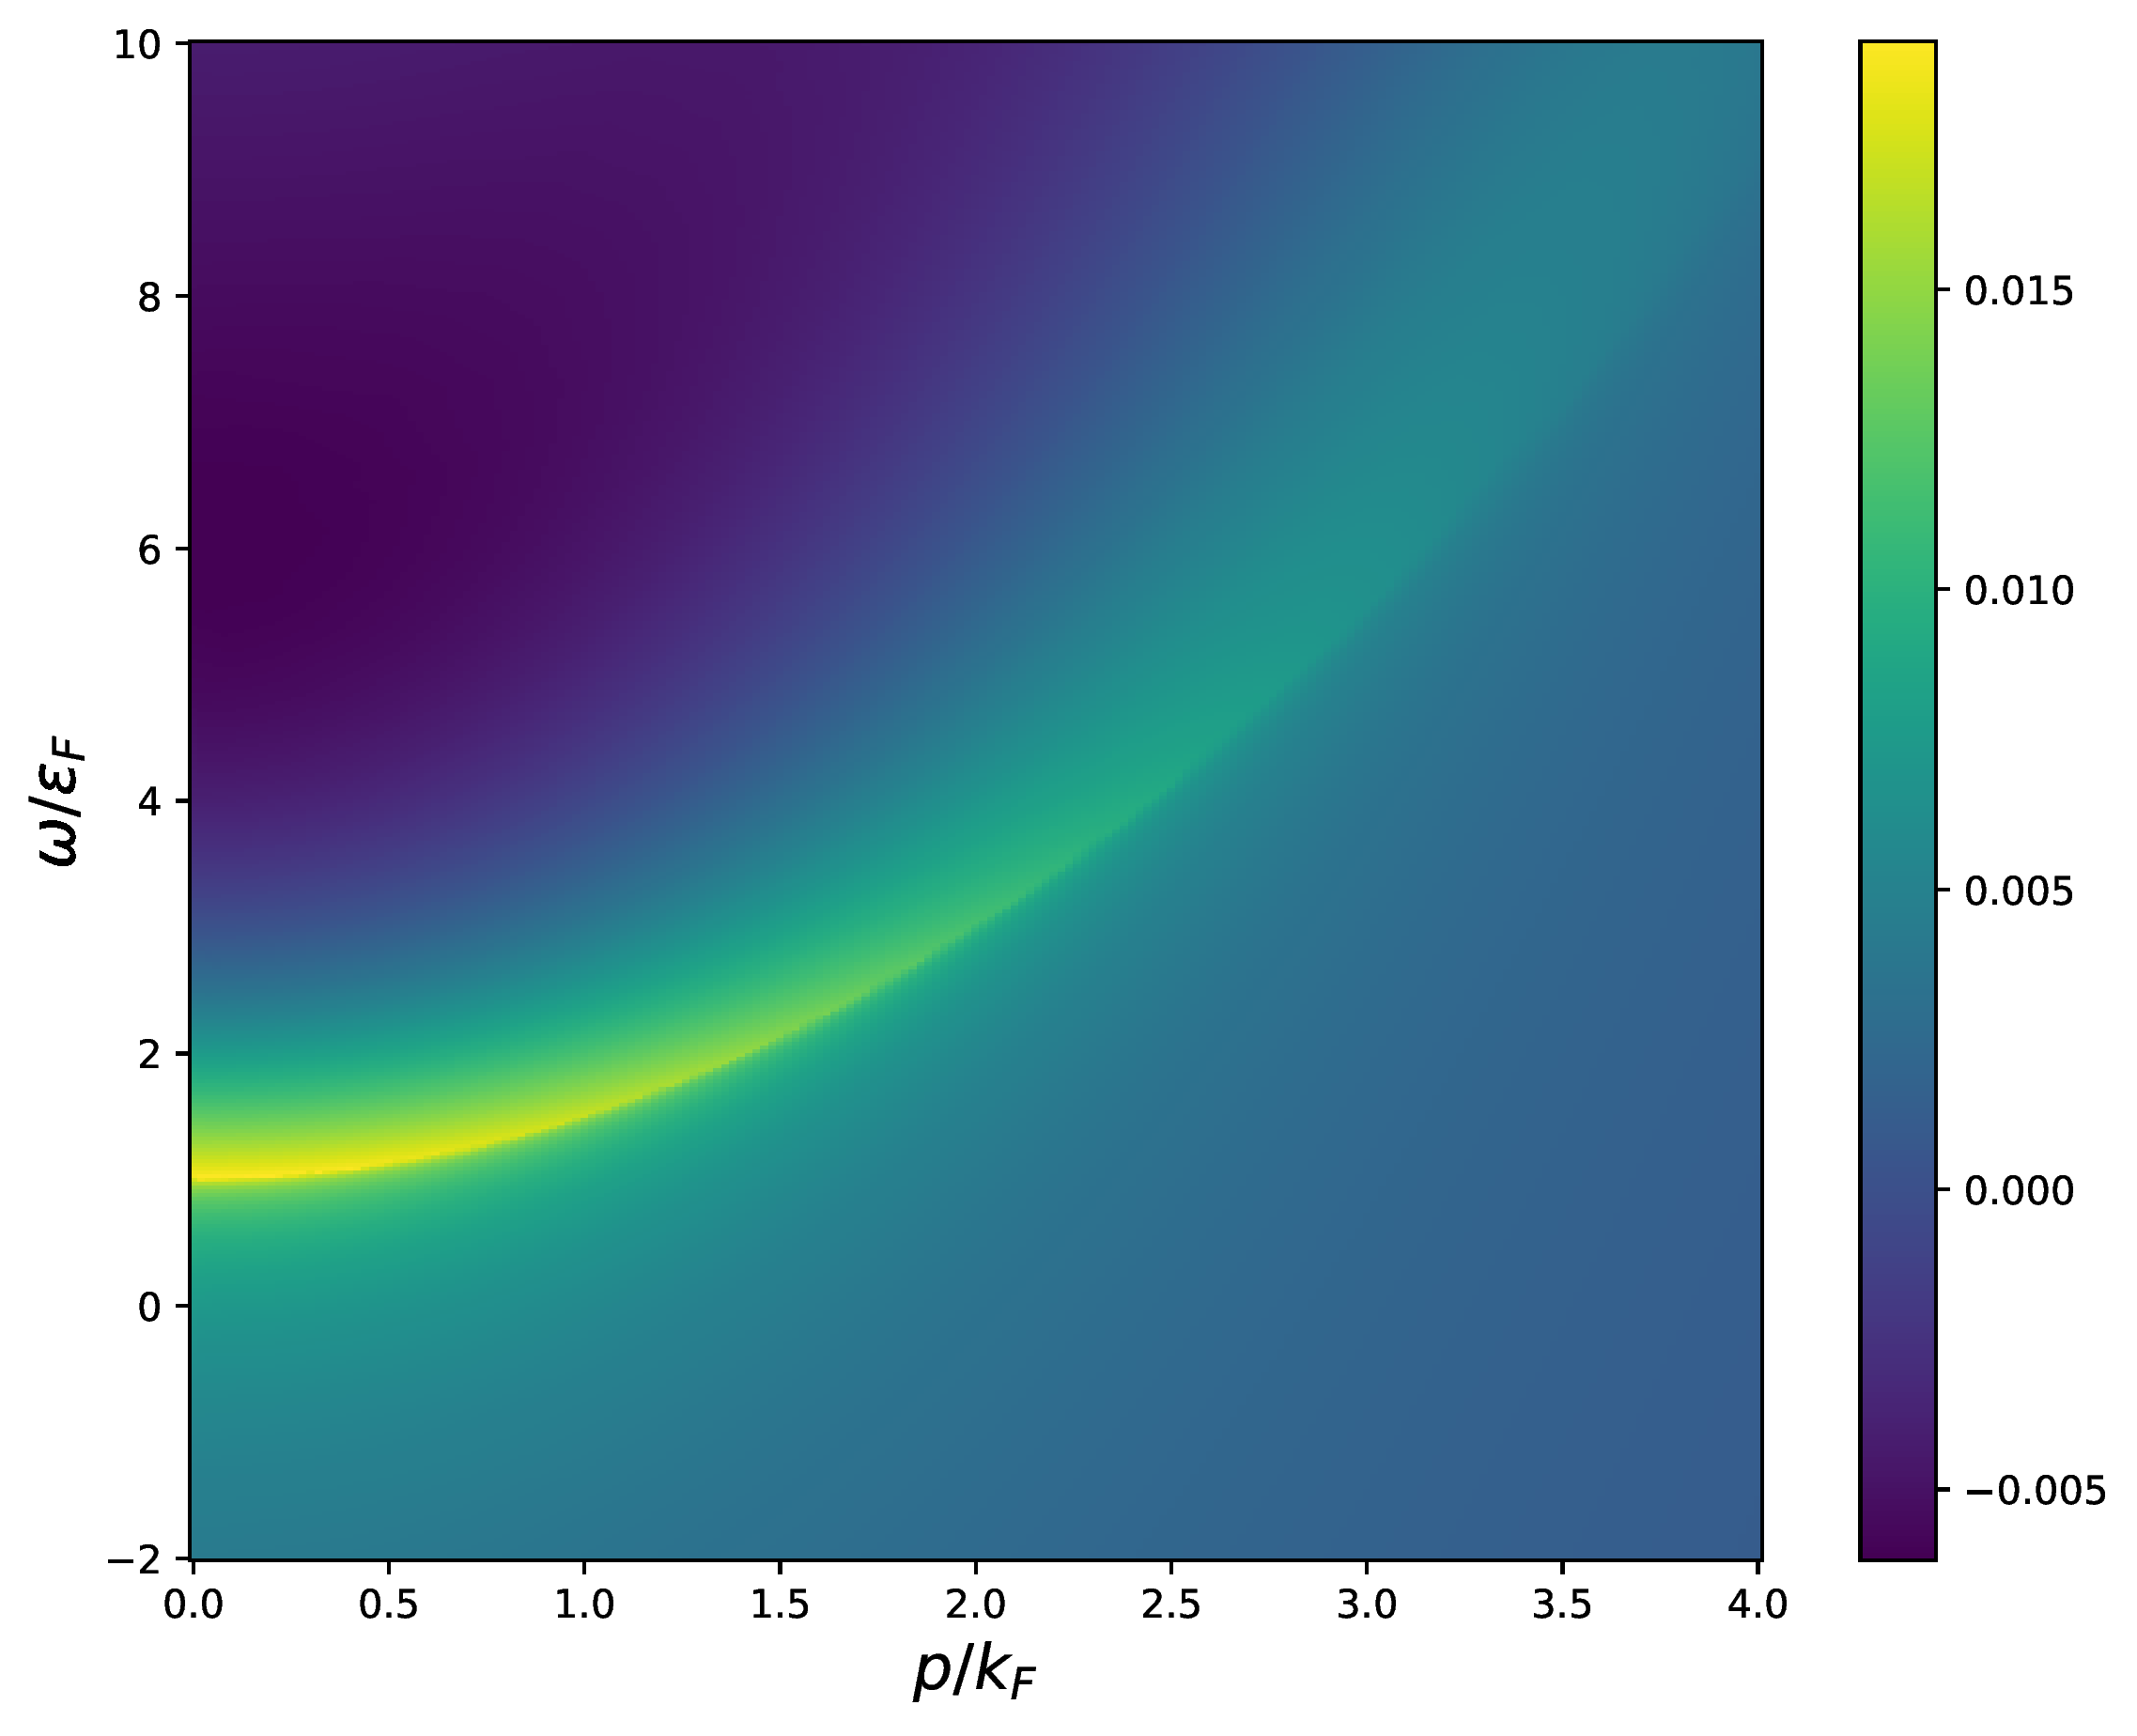
\includegraphics[width=0.46\textwidth]{figs/dispersion-shift2.png}}
	\caption[Improving sampling and interpolation of 2d functions with sharp edges]{Procedure to improve the interpolation of sharp edges and curvy functions. (a) A 2-dimensional function is transformed onto the dispersion relation and linearly interpolated $f(\omega,\bm{p})$. (b) Afterwards, the interpolated function is shifted back to the dispersion relation $f(\omega-\bm{p}^2/2,\bm{p})$.}
	\label{fig:shift_dispersion}
\end{figure}


%%%%%%%%%%%%%%%%%%%%%%%%%%%%
\subsection*{Boson spectral function}
\label{subsec:boson_spec}

In this Section, we detail the calculation and representation of the boson spectral function $\rho_{\phi}$. Since the renormalized bosonic self-energy~\eqref{eq:self-energies} includes a counterterm, the numerical procedure requires suitable subtraction schemes and analytic treatment. 

The problematic part is the well-known vacuum solution, which is given by
%
\begin{align}
\Pi^0_{\phi}(\omega_n, \bm{p}) &= h^2 \int_{\bm{q}} \left[\frac{1}{-i\omega_m+\varepsilon_{\bm{q}}+\varepsilon_{\bm{p-q}}-2\mu} - \frac{1}{2\varepsilon_{\bm{q}}}\right] \notag \\
&= \frac{h^2}{8\pi} \sqrt{-\frac{i\omega_n}{2}+\frac{\bm{p}^2}{4}-\mu}  \,.
\end{align}
%
This means that the vacuum part,
%
\begin{align}
\mathrm{Im}\,\Pi^{R,0}_{\phi}(\omega, \bm{p}) = \frac{h^2}{8\pi} \sqrt{\frac{\omega}{2}-\frac{\bm{p}^2}{4}+\mu}  \,,
\end{align}
%
can be subtracted from the total numerical self-energy $\mathrm{Im}\,\Pi^{R}_{\phi}(\omega, \bm{p})$ in order to treat the divergent real part analytically. Thus, we calculate the full numerical imaginary part of the self-energy and obtain the real part via
%
\begin{align}
\mathrm{Re}\,\Pi^{R}_{\phi}(\omega, \bm{p}) &= \mathrm{Re}\,\Pi^{R,0}_{\phi}(\omega, \bm{p}) \notag \\
&+ \frac{1}{\pi} \int_{\lambda} \frac{\mathrm{Im}\,\Pi^R_{\phi}(\lambda,\bm{p})-\mathrm{Im}\,\Pi^{R,0}_{\phi}(\lambda,\bm{p})}{\lambda-\omega} \,,
\end{align}
%
where $\mathrm{Re}\,\Pi^{R,0}_{\phi}(\omega, \bm{p})$ is the real part of the vacuum solution
%
\begin{align}
\mathrm{Re}\,\Pi^{R,0}_{\phi}(\omega, \bm{p}) = -\frac{h^2}{8\pi} \sqrt{-\frac{\omega}{2}+\frac{\bm{p}^2}{4}-\mu} \,.
\end{align}
%
With these formulas, we can obtain $\mathrm{Im}\,\Pi^{R}_{\phi}$ and $\mathrm{Re}\,\Pi^{R}_{\phi}$ on a finite grid numerically.

However, the calculation of the real part requires also information about the high frequency tails outside the numerical grid. In this case, the imaginary part outside the grid is approximated by the analytic formula of the non-selfconsistent self-energy discussed in the previous Section,
%
\begin{align}
\mathrm{Im}\,\Pi^{R}_{\phi}(\omega, \bm{p})-\mathrm{Im}\,\Pi^{R,0}_{\phi}(\omega, \bm{p}) \approx \mathrm{Im}\,\Pi^{R,T}_{\phi}(\omega, \bm{p}) \,,
\end{align}
%
for large $\omega$. Thus, the bosonic spectral function outside the grid is approximated by the non-selfconsistent spectral function $\rho^{(1)}_{\phi}$ (first iteration). A different subtraction scheme would be to subtract the whole non-selfconsistent imaginary part straightaway and only deal with differences to the first iteration. In principle, both methods are equivalent and work similar. For practical reasons, we choose the latter subtraction scheme.

Another trick to improve the numerical calculation was already mentioned above. Since the boson self-energy follows a quadratic dispersion relation, it is practical to transform the functions onto the dispersion relation before interpolation, as shown in Fig.~\ref{fig:shift_dispersion}. This way, a better sampling and interpolation of the important regions can be achieved. Afterwards, the interpolated function is shifted back to the correct dispersion relation.

Since the fermion spectral functions in the self-energy integrals are very peaked for lower temperatures and larger momenta, it might be useful to subtract a broadened classical spectral function, or the first iteration, from the further iterations in order to improve the integration for larger momenta. The contribution from the subtracted spectral function has then to be taken into account. Since the fermion spectral functions are represented on a finite numerical grid, the bare delta peak contributions from outside the grid has to be taken into account too. This is similar to the peak-tail splits from~\cite{Horak2019}.

For the representation of the numerical self-energy on the finite grid, an adaptive grid is chosen for the imaginary and real part, separately. The boundaries in frequency are $\omega=(-100,100)\,\varepsilon_F$ and in momentum $p=(0,10)\,k_F$. Approximately 10.000 grid points are needed to obtain stable numerical results.


%%%%%%%%%%%%%%%%%%%%%%%%%%%%
\subsection*{Calculation of the real part via Kramers-Kronig}
\label{subsec:real-part}

It turns out that the calculation of the real part via Kramers-Kronig relation is very sensitive to the high frequency tails of the imaginary part. It is not sufficient to know the imaginary part on a finite grid, but rather, we have to extrapolate the high frequency behavior and estimate its contribution. For constant momentum $p$, the large-frequency behavior of the self-energy $\mathrm{Im}\,\tilde{\Sigma}^{R}(\omega)$ outside the numerical grid is well described by the power law
%
\begin{align}
\mathrm{Im}\,\tilde{\Sigma}^{R}(\omega) \approx \frac{a}{\omega^b} \,,
\end{align}
%
where the constants $a,b$ are determined by a fitting routine. From this fit one can calculate the missing contribution $\delta\mathrm{Re}\,\tilde{\Sigma}^{R}(\omega)$ for the real part at frequency $\omega$. We express the imaginary part as $\mathrm{Im}\,\tilde{\Sigma}^{R}(\lambda) = \mathrm{Im}\,\Sigma^{R}(\lambda)\theta(\omega_{\mathrm{max}}-\lambda) + a\lambda^{-b} \theta(\lambda-\omega_{\mathrm{max}})$ with a contribution inside and outside the numerical grid with frequency cutoff $\omega_{\mathrm{max}}$. From the Kramers-Kronig relation, we obtain the contribution outside the grid
%
\begin{align}
	\delta\mathrm{Re}\,\tilde{\Sigma}^{R}(\omega) = \int_{\Delta}^{\infty}\frac{\mathrm{Im}\,\tilde{\Sigma}^{R}(\omega+\lambda)\,d\lambda}{\pi\lambda} = \int_{\Delta}^{\infty}\frac{a\,d\lambda}{\pi\lambda(\omega+\lambda)^b} \,,
\end{align}
%
where $\Delta=\omega_{\mathrm{max}}-\omega$. Evaluating the last integral gives the analytic expression
%
\begin{align}
\delta\mathrm{Re}\,\tilde{\Sigma}^{R}(\omega) = \frac{a}{\pi\Delta^b b}\,{}_{2}F_{1}\left(b,b;1+b;-\frac{\omega}{\Delta}\right) \,,
\end{align}
%
where ${}_{2}F_{1}\left(a,b;c;z\right)$ is the hypergeometric function~\cite{Abramowitz1972}. Using this large-frequency contribution from outside the grid, improves the determination of the real part significantly. For the fermion self-energy, we observe $b\approx 0.5$ for large enough $\omega_{\mathrm{max}}$.

This asymptotic behavior can be shown by similar arguments as in Ref.~\cite{Schneider2009}. We consider only the large frequency behavior and rewrite the imaginary part of the fermion self-energy in~\eqref{eq:imaginary-part-self-energies} as
%
\begin{align}
	\mathrm{Im}\,\Sigma^R_{\psi}(\omega) \sim \int_{\bm{q},\lambda_1,\lambda_2}
	\rho_{\phi}(\lambda_1) \rho_{\psi}(\lambda_2)
	\delta(\omega-\lambda_1+\lambda_2) \left[n_B(\lambda_1)+n_F(\lambda_2)\right] \,.
\end{align}
%
In the limit $\omega\rightarrow\infty$, the delta function only contributes if (a) $\lambda_1$ large and $\lambda_2$ small or (b) $\lambda_2$ large negative and $\lambda_1$ small. In case (b), however, the fermion spectral function $\rho_{\psi}$ vanishes for small momenta and $\lambda_2\rightarrow-\infty$. Thus, only case (a) contributes and we are left with
%
\begin{align}
\mathrm{Im}\,\Sigma^R_{\psi}(\omega) \sim \int_{\bm{q},\lambda_2} \rho_{\phi}(\omega+\lambda_2) \rho_{\psi}(\lambda_2) n_F(\lambda_2) \,,
\end{align}
%
where we have used $n_B(\lambda_1)\rightarrow 0$ for $\lambda_1\rightarrow\infty$. As seen above, the large frequency behavior of the boson spectral function is dominated by $\rho_{\phi}(\omega)\sim 1/\sqrt{\omega}$. Additionally, the integrand vanishes for large negative values of $\lambda_2$, since $\rho_{\psi}(\lambda_2)$ vanishes, and for large positive values of $\lambda_2$, since $n_F(\lambda_2)$ vanishes. Thus, the range of $\lambda_2$ is limited and we can write
%
\begin{align}
\mathrm{Im}\,\Sigma^R_{\psi}(\omega) \sim \int_{\bm{q},\lambda_2} \rho_{\psi}(\lambda_2) n_F(\lambda_2) / \sqrt{\omega} \sim 1/\sqrt{\omega} \,,
\end{align}
%
where we used that $\int_{\bm{q},\lambda_2} \rho_{\psi}(\lambda_2) n_F(\lambda_2) = n$ is finite in the last step.


With the same argument one can show that $\mathrm{Im}\,\Sigma^R_{\psi}(\omega)$ vanishes rapidly for large negative frequency. 



%%%%%%%%%%%%%%%%%%%%%%%%%%%%
\subsection*{Iterative procedure}
\label{subsec:iteration}

Using~\eqref{eq:imaginary-part-self-energies} and the Kramers-Kronig relation, the retarded self energies can be computed in every iteration step and fed back into the next, after extraction of the spectral function via~\eqref{eq:spectral-relation}. The iterative procedure is initialized with the classical fermion spectral function,
%
\begin{align} \label{eq:inital-fermion-spec}
\rho^{(0)}_{\psi}(\omega,\bm{p}) = \delta(\omega-\bm{p}^2+\mu) \,.
\end{align}
%
This initial guess is inserted into the spectral form of $\Pi_{\phi}$ to obtain the first iteration of the boson spectral function $\rho_{\phi}^{(1)}$. Then, $\rho_{\phi}^{(1)}$ together with $\rho^{(0)}_{\psi}$ are inserted into the spectral integral of $\Sigma_{\psi}$ to obtain the first iteration of the fermion spectral function $\rho_{\psi}^{(1)}$. Now, $\rho_{\psi}^{(1)}$ can be used to obtain the next iteration for the boson spectral function $\rho_{\phi}^{(2)}$, and so on. In general, $\rho_{\psi}^{(i)}$ is used to obtain $\rho_{\phi}^{(i+1)}$, and $\rho_{\phi}^{(i+1)}$ and $\rho_{\psi}^{(i)}$ are used to obtain $\rho_{\psi}^{(i+1)}$. This iteration is repeated until convergence is reached. We observe that around 5-20 iterations are needed to obtain a converged result with ($\Lambda$: numerical momentum cutoff)
%
\begin{align}
\int_{\bm{q},\lambda}^{\Lambda} \left| \rho^{(i)}(\lambda,\bm{q})-\rho^{(i-1)}(\lambda,\bm{q}) \right| \lesssim 0.005\, \Lambda \,.
\end{align}
%
This criterion is similar to the statement that, at this point, the density $n^{(i)}$ obtained from the $i$th iteration does not change significantly anymore. In our case, the accuracy is around $1\%$.
As mentioned in the main text, the convergence is worse closer to the critical temperature and the spectral functions may jump around. One can improve the convergence by iterating twice over the fermions or updating the spectral functions only partially. Other methods are discussed in the main text.